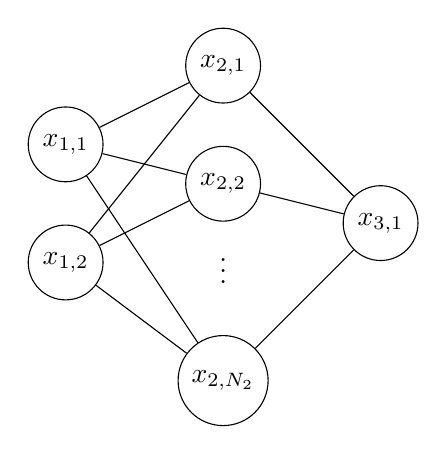
\begin{tikzpicture}
    \tikzstyle{neuron}=[draw,circle];
    \node (x11) [neuron] at (-2,1.5) {$x_{1,1}$};
    \node (x12) [neuron] at (-2,0) {$x_{1,2}$};
    \node [neuron] (x21) at (0,2.5) {$x_{2,1}$};
    \node [neuron] (x22) at (0,1) {$x_{2,2}$};
    \node (x23) [neuron] at (0,-1.5) {$x_{2,N_2}$};
    \node (x31) [neuron] at (2,0.5) {$x_{3,1}$};
    \node at (0,0) {$\vdots$};
    
    \foreach \i in {1,2}{
        \foreach \j in {1,2,3}{
            \draw (x1\i) -- (x2\j);
        }
    }
    
    \foreach \j in {1,2,3}{
        \foreach \k in {1}{
            \draw (x2\j) -- (x3\k);
        }
    }
    
\end{tikzpicture}